%       %======================================================================
%       %  Section
%       %======================================================================
        \section{ボイルの法則}
            近代科学の先駆者としてコペルニクス
                \footnote{
                    Nicolaus Copernicus (1473--1543,?):地動説を唱えたことで有名.
                    地球は太陽を中心に公転しているのだ.
                }
            やガリレイがよく挙げられる.
            それ以前には,思考のみによって世界の真理を追求してきたのだが,
            彼らは,これに疑問を訴え,観察や実験を通した事実を基に,世界の真理を
            追求すべきだと主張した.

            ボイル
                \footnote{
                    Robert Boyle (1627--1691,イギリス):化学者,物理学者.
                }
            もその考えに基づき, \textbf{自然を実験と観察に基づいて考える} という理念の下で,
            主に化学現象に関する研究を行っていた.
            その中で,ボイルは気体に関する法則を
            実験的に見出した.\textbf{ボイルの法則} である.
                \begin{myshadebox}{ボイルの法則}
                    温度を一定に保っている状態では,圧力と体積は反比例の関係にある.
                    言い換えると,圧力と体積の積は一定値を保つ.
                    圧力を $p$,体積を $V$ としたとき,
                    \begin{align}
                        pV = k. \mbox{(温度一定)}
                    \end{align}
                    ここで,$k$ は気体の初期状態により決まる定数.
                \end{myshadebox}

            ボイルの法則や,この後に説明するシャルルの法則は,熱力学の教科書だけでなく,
            化学の教科書にも登場する.その意味で,熱力学と化学を結ぶ重要な法則である.


%       %======================================================================
%       %  Section
%       %======================================================================
        \section{シャルルの法則}
            シャルル
                \footnote{
                    Jacques Alexandre C\'{e}sar Charles (1746--1823):化学者.
                }
            気体に関する法則を実験的に見出した.\textbf{シャルルの法則} とよばれる.
                \begin{myshadebox}{シャルルの法則}
                    圧力を一定に保っている状態では,体積と温度は比例関係にある.
                    言い換えると,体積と温度の比は一定値を保つ.
                    体積を $V$,温度を $T$ としたとき,
                    \begin{align}
                        \frac{V}{T} = l. \mbox{(圧力一定)}
                    \end{align}
                    ここで,$l$ は気体の初期状態により決まる定数.
                \end{myshadebox}

            比例定数についても実験的に得られる.もう少しシャルルの法則を詳しく書くと,
            次よようになる.すなわち,\textbf{一定圧力において,気体の体積は,
            温度を1度上昇させると,0度の時の体積の1/273ずつ増加する}.
            式で表すと,0度の時の体積を ${V}_{0}$ とし,温度t度上昇させた時の,気体の体積 $V(t)$ は,
                \begin{equation*}
                    V(t) = \frac{1}{273} {V}_{0}t + {V}_{0}.
                \end{equation*}
            次のように式変形してみよう.
                \begin{equation*}
                    V(t) = \left( \frac{1}{273}t + 1 \right) {V}_{0} = \frac{t+273}{273} {V}_{0}.
                \end{equation*}
            $T=t+273$ を導入して,
                \begin{equation*}
                    V(t) = \frac{T}{273} {V}_{0}
                \end{equation*}
            となる.この $T$ のことを \textbf{絶対温度} といい,単位を [K] で表す.
            [K] は「ケルビン」と読む.
                \begin{figure}[hbt]
                    \begin{center}
                        \includegraphicsdefault{charlesNohousoku.pdf}
                        \caption{シャルルの法則}
                        \label{fig:charlesNohousoku}
                    \end{center}
                \end{figure}


%       %======================================================================
%       %  Section
%       %======================================================================
        \section{ボイル$=$シャルルの法則}
            ボイルの法則とシャルルの法則を1つにまとめることができる.
            ひとまとめにできることを示すには,実際に状態遷移の計算をしてみて,
            矛盾がないことを確認すればいい.

            温度 $T$ と体積 $V$ と圧力 $p$ の添字のアルファベット(A, B, C)は,
            図\ref{fig:BoyleCharlesTotal1111}で示す状態に対応する.
            状態遷移は次のように行う.まず,最初の状態をAとする.状態Aから
            等温変化させて,状態Bへ移す.この時,等温変化であるから,ボイルの
            法則が成り立つはずである.更に,状態Bから状態Cへ等圧変化により
            遷移させる.この場合は,等圧変化であるので,シャルルの法則が
            成り立つはずである.最後に,状態Aと状態Cにおける各温度,体積,圧力
            の関係が等しければ,ボイルの法則とシャルルの法則をひとまとめに
            できることが示される.
            \begin{figure}[hbt]
                \begin{center}
                    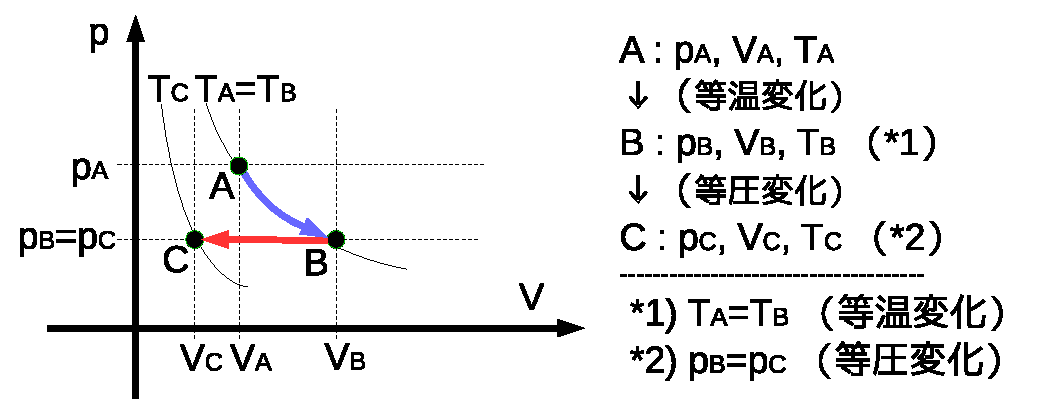
\includegraphics[keepaspectratio, width=8.0cm,height=3.3cm,clip]{BoyleCharlesTotal1111.pdf}
                    \caption{ボイル$=$シャルルの法則}
                    \label{fig:BoyleCharlesTotal1111}
                \end{center}
            \end{figure}

            一定温度 $T_{A}$ の下で,ボイルの法則により,
                \begin{equation*}
                    {p}_{A}{V}_{A} = {p}_{B}{V}_{B}.
                \end{equation*}
            後の式変形のため,${V}_{B}$ について解いておく.
                \begin{equation*}
                    {V}_{B} = \frac{{p}_{A}{V}_{A}}{{p}_{B}}.
                \end{equation*}

            引き続き,一定圧力 $p_{B}$ の下で,シャルルの法則より,
                \begin{equation*}
                    \frac{{V}_{B}}{{T}_{B}} = \frac{{V}_{C}}{{T}_{C}}.
                \end{equation*}
            ${V}_{B}$ を置き換えて,
                \begin{equation*}
                    \frac{{p}_{A}{V}_{A}}{{T}_{B}{p}_{B}} = \frac{{V}_{C}}{{T}_{C}}.
                \end{equation*}
            両辺に ${p}_{B}$ をかけておく.
                \begin{equation*}
                    \frac{{p}_{A}{V}_{A}}{{T}_{B}} = \frac{{p}_{B}{V}_{C}}{{T}_{C}}.
                \end{equation*}

            ここで,状態AからBの遷移は等温変化であるので,
                \begin{equation*}
                    {T}_{B} = {T}_{A}.
                \end{equation*}
            また,状態Bから状態Cへの遷移は等圧変化であるので,
                \begin{equation*}
                    {p}_{B} = {p}_{C}.
                \end{equation*}
            この2点を考慮すると
                \begin{equation*}
                    \frac{{p}_{A}{V}_{A}}{{T}_{A}} = \frac{{p}_{C}{V}_{C}}{{T}_{C}}.
                \end{equation*}
            式の添字に着目すれば,最初の状態Aと最後の状態Cにおいて,
            関係式 $pV/T$ が同じ値をとることがわかる.この値を $k$ と書くことにすれば
                \footnote{
                    \begin{equation*}
                        k := \frac{{p}_{A}{V}_{A}}{{T}_{A}} = \frac{{p}_{C}{V}_{C}}{{T}_{C}}.
                    \end{equation*}
                },
                \begin{equation*}
                    \frac{pV}{T} = k.
                \end{equation*}
            次のように書き換えれば,よく見かける方程式になる.
                \begin{equation*}
                    pV=kT.
                \end{equation*}
            これが,\textbf{ボイル$=$シャルルの法則} である.
            ボイル$=$シャルルの法則の式は,\textbf{気体の状態方程式} とよばれる.

            まとめておこう.
                \begin{myshadebox}{ボイル$=$シャルルの法則}
                    気体において,温度 $T$,体積 $V$,圧力 $p$ は,
                    定数 $k$ を用いて,以下の関係式を満たす.
                    \begin{align}
                        pV=kT.
                    \end{align}
                \end{myshadebox}

%       %======================================================================
%       %  Section
%       %======================================================================
        \section{理想気体}
        理想気体の状態方程式が厳密に成り立つ理想的な気体のことを \textbf{理想気体} という.
        理想気体は実在しないが,高温状態あるいは低圧状態では,実在する気体を理想気体と
        みなしうることができる,ということもある.実際は,工学的には,理想と現実の乖離具合
        を常に意識しなければならない.ただ,理論構築のためには,理想気体はとても
        有用なので,熱力学では理想気体が主役になる.理想気体の性質を理論的に把握することで,
        現実に存在する \textbf{実在気体} の性質を推察できるようになる.
        どれだけ実在気体が理想気体と乖離しているかが,実在気体の特徴であるともいえる.

%       %======================================================================
%       %  Section
%       %======================================================================
        \section{状態方程式}
        \begin{mycomment}
            気体が従う自然法則(方程式)を導入する.
            熱力学では,ニュートンの運動方程式と同じように,天下り的に与えられる式であり,他から導き出されるものではない.
            気体を無数の粒子の集まりとして仮定した統計力学から,理想気体の状態方程式を導けるが,これは熱力学の論理の範囲外である.
            今は熱力学を学習しているため,状態方程式は実験事実の自然法則として受け入れよう.
        \end{mycomment}
        \subsection{理想気体の状態方程式}
        状態方程式は熱力学の基本法則の1つである.以下に書き下そう.
        \begin{myshadebox}{理想気体の状態方程式}
            理想気体において,圧力$P$[N/m${}^{2}$],体積$V$[m${}^{3}$],物質量$n$[mol], 温度$T$[K],
            気体定数$R$[J/mol$\cdot$K]の条件下で,以下が成り立つ.
            \begin{equation}
                PV = nRT.
            \end{equation}
        \end{myshadebox}

        理想気体の状態方程式のことは,混乱の恐れがない場合には,単に,状態方程式ともいう.

        \subsection{気体の濃度}
        体積$V$[m${}^{3}$]の容器の中に$n$[mol]の気体が入っているとき,この気体の濃さを
        数値化できる.同じ堆積中で,たくさん気体が入っていれば濃くなるし,少なければ,
        薄くなる.これを \textbf{濃度} という.濃度を$\sigma$で現すと,
            \begin{align}
                \sigma = \frac{n}{V}
            \end{align}
        である.状態方程式と対比させてみと,以下になる.
            \begin{align*}
                 PV &= nRT \\
                \Leftrightarrow P &= \frac{n}{V}RT \\
                \Leftrightarrow P &= \sigma RT \\
            \end{align*}

        濃度$\sigma = n/V$が一定の場合に成立する式だ.圧力は濃度に比例する.
        気体の濃度が濃いほど圧力は高くなるのだ.
        \begin{align}
            P(T) = \sigma RT.
        \end{align}

        注意すべきは式を濃度$\sigma$について解いてみて
        \begin{align}
            \sigma = \frac{P}{RT}
        \end{align}
        としてしまうと,あたかも濃度が圧力に比例するようにみえる.この解釈は間違いである.
        濃度はもともと,$n/V$であることを忘れてはいけない.$n$の値は変化しない(急に気体が湧いて出たりしない).
        つまり,圧力が変化して濃度が変わったのであれば,実際には体積$V$が変化したということである.
        圧力$P$を高くして体積$V$をぐぐっと縮みることで,濃度が高くなるのだ.

        \subsection{実在気体の状態方程式}
        \subsubsection{ビリアル方程式}
        \subsubsection{ファンデルワールスの状態方程式}
        実在する気体の振る舞いをいい感じに表現する方程式がある.液体にも適用可能である.
        ファンデルワールス
            \footnote{
                Johannes Diderik van der Waals(1837--1923,オランダ):ヨハネス ディーデリク ファン デル ワールス.
                1910年にこの気体の状態方程式の発見によりノーベル賞を受賞している.分子間力の1つである,
                \textbf{ファンデルワールス力}(\textbf{ファンデルワールス結合})でもその名前が知られている.
            }というオランダ人の物理学者が提案した,実在気体の状態方程式である.
        気体の種類によって,振る舞いが異なるので,それに対応する特徴的な 定数$a$,$b$が使われる.

        ファンデルワールスの状態方程式も他から導かれるものではないが,雰囲気からなら説明・導入ができる.
        理想気体の状態方程式に現実的要素を織り交ぜて,変形していく.理想気体からの乖離を補正するのである.
        補正を受けるのは,体積$V$と圧力$P$である.まず,体積から考えよう.

        理想気体を構成する粒子は体積はないものと仮定されていた
            \footnote{
                実際,熱力学が成立した時代にも,原子や分子の存在は知られていなかった.
                確かに,デモクリトストスが提唱していたと言われているが,空想上の概念であり,
                デモクリトスが実験的に原子や分子の存在を確かめたわけではない.
            }.
        しかし,実在気体を構成する粒子は,一つ一つは微小であるが,体積を持つ.
        現実気体$n$[mol]の体積を${V}_{R}$(RealのR),おなじく理想気体$n$[mol]の体積を${V}_{I}$(ImageのI)とするならば,
        体積の補正項を$b$を導入して,
            \begin{equation}
                {V}_{R} = {V}_{I} + bn
            \end{equation}
        と書ける.実在気体の体積は理想気体の体積よりも,粒子自体の大きさ分だけ,大きいと考える.
        \begin{figure}[hbt]
            \begin{center}
                \includegraphicsmiddle{netsurikigaku_van_der_waals_force.pdf}
                \caption{実在気体:体積}
                \label{fig:netsurikigaku_van_der_waals_force}
            \end{center}
        \end{figure}

        実在の気体の圧力も理想とは異なる.実際には分子を構成する原子機構により分子内部の電子の位置が偏り,
        分子自体に正負の電気的な偏りができる.これが複数存在すると,分子のプラス側(正)と別の分子のマイナス側(負)が
        引き合う現象がおきる.これを \textbf{分子間力} という
            \footnote{
                分子間力といっても,発生機構によって細分化される.イオン間相互作用,水素結合,双極子相互作用,ファンデルワールス力.
            }.
        分子間力が働くと,分子の運動が束縛されて(分子の運動が鈍くなり),結果,圧力が弱まる.
        \begin{figure}[hbt]
            \begin{center}
                \includegraphicsmiddle{netsurikigaku_van_der_waals_force2.pdf}
                \caption{実在気体:圧力}
                \label{fig:netsurikigaku_van_der_waals_force2}
            \end{center}
        \end{figure}
        では,どの程度弱まるのか.モル濃度の2乗に比例すると考えられている(根拠は実験かな).
        現実気体$n$[mol]の圧力を${P}_{R}$(RealのR),おなじく理想気体$n$[mol]の圧力を${P}_{I}$(ImageのI)とするならば,
        圧力の補正項を$a$を導入して,
        \begin{equation}
            {P}_{R} = {P}_{I} - a{\left( \frac{n}{{V}_{I}} \right)}^{2}
        \end{equation}
        となる.

        理想気体の状態方程式は厳密に成り立つ.${V}_{I}$と${P}_{I}$を使って理想気体の状態方程式を書くならば,
        \[
            {P}_{I}{V}_{I} = nRT.
        \]
        だけど,${V}_{I}$と${P}_{I}$は実在気体の体積と圧力だから,この式は間違っている.式を補正して正しくしよう.
        この理想気体型の状態方程式に,さっき計算した結果を適用すればよい.
        まず,上記の2つの式をそれぞれ,${V}_{I}$と${P}_{I}$について解くと,
        \begin{align}
            {V}_{I} &= {V}_{R} - bn \\
            {P}_{I} &= {P}_{R} + a{\left( \frac{n}{{V}_{I}} \right)}^{2}
        \end{align}
        である.これを状態方程式に代入しよう.
        \begin{equation}
            \left( {P}_{I} + a{\left( \frac{n}{{V}_{I}} \right)}^{2} \right) \left( {V}_{I} - bn \right) = nRT.
        \end{equation}
        カッコが多くてきたないので,適当に外すと,
        \begin{equation}
            \left( {P}_{I} + a\frac{{n}^{2}}{{{V}_{I}}^{2}} \right) \left( {V}_{I} - bn \right) = nRT.
        \end{equation}
        となる.

        これを \textbf{ファンデルワールスの状態方程式} という.
        また,$a$,$b$のことを \textbf{ファンデルワールス定数} という.
        \begin{myshadebox}{ファンデルワールスの状態方程式}
            現実気体$n$[mol]の圧力を${P}_{I}$,現実気体$n$[mol]の体積を${V}_{I}$として(RealのR),
            \begin{equation}
                \left( {P}_{I} + a\frac{{n}^{2}}{{{V}_{I}}^{2}} \right) \left( {V}_{I} - bn \right) = nRT.
            \end{equation}
        \end{myshadebox}

        「理想気体の圧力に対して,実在気体の圧力は分子間力の分だけ小さくなるので,補正項を足す」,
        「理想気体の体積に対して,実在気体の体積は大きさがある分だけ大きくなるので,補正項を引く」
        と捉えておけばよいだろう.

        ちなみに,教科書には${P}_{I}$を左辺にした表現となっていた.
        \begin{equation}
             {P}_{I}  =  \frac{nRT}{\left( {V}_{I} - bn \right)} - a{\left(\frac{n}{{V}_{I}} \right)}^{2}.
        \end{equation}
        ちょっと細工すると,
        \begin{equation*}
            {P}_{I}  =  \frac{1}{\left( {V}_{I} - bn \right)}nRT - a{\left(\frac{n}{{V}_{I}} \right)}^{2}.
       \end{equation*}
        この表現からは,現実気体の圧力は,理想気体の$1/({V}_{I} - bn)$で,さらに,分子間力がはたらく分だけ
        小さくなることが読み取りやすい.

%       %======================================================================
%       %  Section
%       %======================================================================
        \section{分圧の法則}
        混合気体が入った容積の圧力を考える.この容積内部の圧力について,以下の法則が成り立っている.
        \begin{myshadebox}{分圧の法則}
            混合気体の圧力(全圧)は,それを構成する各々の種類の成分圧力(分圧)
            の和に等しい.気体は何種類もあってよくて,$k$種類の気体がある場合は
            以下の式が成り立つ.
            \begin{equation}
                P = \sum_{i=1}^{k} {p}_{i}
            \end{equation}
            左辺の$P$が全圧であり,右辺の${p}_{i}$($i=1,\,2,\,\cdots,\,n$)が分圧である.
        \end{myshadebox}
        ドルトンが提唱した法則なので,「ドルトンの分圧の法則」とかと紹介されることも多い.

        \begin{figure}[hbt]
            \begin{center}
                \includegraphicsmiddle{netsurikigaku_bunsi_undo_ron_bunatsu.pdf}
                \caption{全圧と分圧}
                \label{fig:netsurikigaku_bunsi_undo_ron_bunatsu}
            \end{center}
        \end{figure}

        う〜ん,この法則はどうやって実験的に確かめたのだろうか.
        原理的には,こうだろう.まず,同体積の気体A,B,Cを用意して,
        それぞれの圧力の計測する.これは,後で気体を混合した場合に,元々の各気体の分圧の測定とみなせる.
        その結果をそれぞれ${P}_{A}$,${P}_{B}$,${P}_{C}$であったとしよう.
        次に,同じ体積ににA,B,Cの3つの気体を同じ一つの箱に押し込めて,圧力を測定する.
        たとえば,BとCをAの箱に詰めるなど.そうすると,3種類の全気体が1箇所に集まることになり,
        このAとBとCから構成される全気体の圧力(すなわち全圧)の測定が可能になる.
        分圧の法則にしたがえば,全圧を単に$P$すると,
            \[
                P = {P}_{A} + {P}_{B} + {P}_{C}
            \]
        と計算できる.

        気体が分子から構成されていることと理想気体の状態方程式から,分圧の法則が導けないだろうか.
        もう少し遊んでみよう.
        
        状態方程式$PV=nRT$から,$P=(n/V)RT$.温度$T$は一定であるとする.すると,
        \[
            \frac{n}{V}RT = \frac{{n}_{A}}{{V}_{A}}RT + \frac{{n}_{B}}{{V}_{B}}RT + \frac{{n}_{C}}{{V}_{A}}RT.
        \]
        ${n}_{A}$,${n}_{B}$,${n}_{C}$はA,B,Cのそれぞれのモル数.
        ${V}_{A}$,${V}_{B}$,${V}_{C}$はそれぞれ,A,B,Cの体積である.体積は同じで,
        \[
            V = {V}_{A} = {V}_{B} = {V}_{C}.
        \]
        だから,
        \begin{align*}
            \frac{n}{V}RT &= \frac{{n}_{A}}{V}RT + \frac{{n}_{B}}{V}RT + \frac{{n}_{C}}{V}RT.
        \end{align*}
        気体の単位体積あたりのモル数(濃度)$\sigma$を考えて,
        \[
            {\sigma}     :=\frac{n}{V},       \quad {\sigma}_{A} :=\frac{{n}_{A}}{V}, \quad
            {\sigma}_{B} :=\frac{{n}_{B}}{V}, \quad {\sigma}_{C} :=\frac{{n}_{C}}{V}
        \]
        と書くことにすると,
        \begin{align*}
                            {\sigma} RT &= {\sigma}_{A} RT + {\sigma}_{B} RT + {\sigma}_{C} RT \\
            \Leftrightarrow {\sigma}    &= {\sigma}_{A}    + {\sigma}_{B}    + {\sigma}_{C}.
        \end{align*}
        となる.体積が一定であれば,それぞれの気体を混ぜ合わせた後の濃度は,それぞれの
        濃度の足し算で計算できる.体積$V$がみえるようにかくと,
        \begin{align*}
                          {\sigma} &= {\sigma}_{A}     + {\sigma}_{B}      + {\sigma}_{C} \\
                       \frac{n}{V} &= \frac{{n}_{A}}{V} + \frac{{n}_{B}}{V} + \frac{{n}_{C}}{V} \\
            \therefore           n &= {n}_{A} + {n}_{B} + {n}_{C}
        \end{align*}
        である.容積中の全体の気体のモル数は,個々の気体のそれぞれのモル数を足し合わせたものである.

        このモル数の足し合わせの結果をベースにして,温度と体積が一定であるという条件の下で,
        これまでの議論を逆にたどれば,分圧の法則が導ける.
        \begin{align*}
                                        n &= \sum_{i=1}^{k} {n}_{i}\\
            \Leftrightarrow \frac{n}{V}   &= \frac{1}{V}\sum_{i=1}^{k} {n}_{i} = \sum_{i=1}^{k} \frac{{n}_{i}}{V}\\
            \Leftrightarrow \frac{n}{V} T &= \left(\sum_{i=1}^{k} \frac{{n}_{i}}{V}\right)  T = \sum_{i=1}^{k}\left( \frac{{n}_{i}}{V} T\right)\\
            \Leftrightarrow \frac{n}{V}RT &= \left(\sum_{i=1}^{k} \frac{{n}_{i}}{V}\right) RT= \sum_{i=1}^{k}\left( \frac{{n}_{i}}{V}RT\right)  \\
            \Leftrightarrow             P &= \sum_{i=1}^{k} {p}_{i}.\quad\mbox{(分圧の法則が導けた)}\
        \end{align*}
        どちらかと言うと,モル数をベースにしたほうが直感的で理解しやすいと思う.ただ,式変形に物理的な洞察はなく,説得力に欠ける.
        モル数をベースにして,温度と圧力が一定だったら,必然的に,分圧の法則が成り立つ,という事実が説明できるだけだ.



